%!TEX root = ../username.tex
% Add your package includes here
\chapter{Design and Implementation of My Digital Wardrobe App}
\label{chap:Chaptert5}
\section{App Development Framework}

The development of this application prioritizes ease of use and efficiency in managing wardrobe items. This chapter walks readers through how the app works, highlighting key features like logging in, uploading images, organizing clothing items, and creating outfits. Since readers may not have direct access to the app, this chapter aims to provide a complete picture of the user experience. It explains how different parts of the app work together behind the scenes. 
\begin{figure}[h]
    \centering
    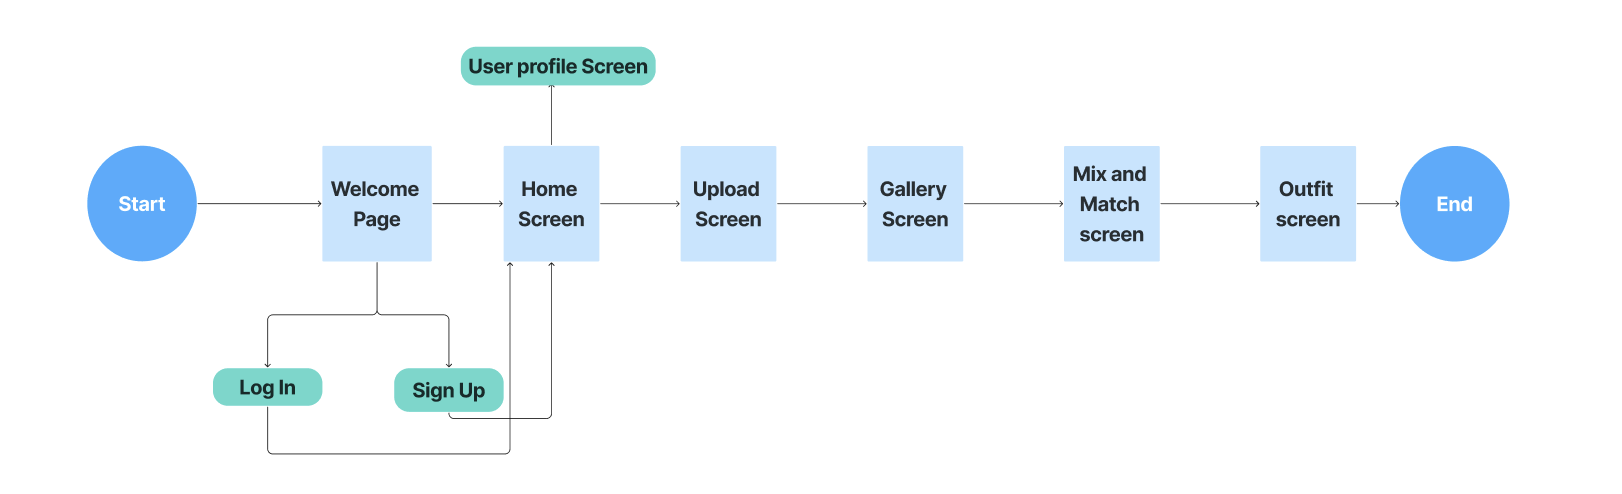
\includegraphics[width=1.1\linewidth]{exampleis-master/figures/updated workflow.png}
    \caption{Screen navigation}
    \label{fig:integration}
\end{figure}

\subsection{Workflow Overview}
The workflow of My Digital Wardrobe outlines how users interact with the app, from signing up to creating and saving outfits. Figure \ref{fig:integration} presents a simplified workflow demonstrating how new users navigate through the app, while  Figure \ref{fig:integration2}  provides a visual representation of this process, highlighting the relationship between user actions, navigation flows, and Firebase services that operate behind the scenes.

\begin{figure}[h]
    \centering
    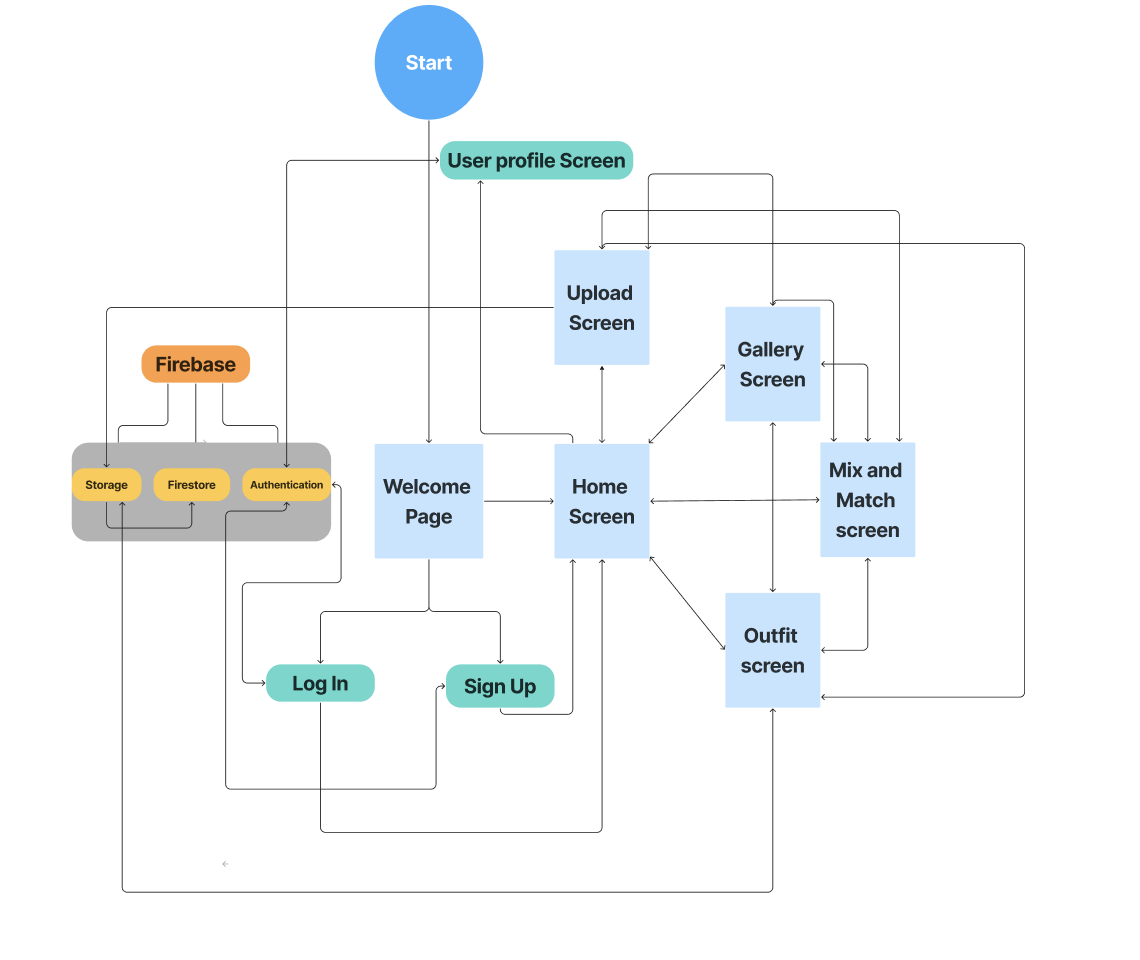
\includegraphics[width=1.0\linewidth]{exampleis-master/figures/updated diagram.png}
    \caption{Workflow diagram}
    \label{fig:integration2}
\end{figure}


At the core of the workflow is the integration between user interactions and backend processes. Users begin at the \textbf{Welcome Page}, where they can either  \textbf{log in} or  \textbf{sign up}. Successful authentication, managed by Firebase, directs users to the  \textbf{Home Screen}, which acts as the central hub. From here, users can navigate to various screens, including the  \textbf{Upload Screen} for adding new wardrobe items, the  \textbf{Gallery Screen} for browsing uploaded clothing, and the  \textbf{Mix and Match Screen}, where outfits can be created and later reviewed on the \textbf{ Outfit Screen}.

Firebase’s services support these interactions. As mentioned in Chapter \ref{chap:Chaptert3},  Authentication verifies user access, Storage handles image uploads, and Firestore organizes metadata for efficient retrieval and categorization. The User Profile Screen is accessible for managing personal information and preferences, ensuring a personalized experience throughout.
This structured workflow ensures that each user action leads to a logical next step, with Firebase managing data storage and access in the background. The navigation between screens is handled dynamically, providing a fluid and intuitive user experience. Further sections will explore each component of this workflow in greater detail, discussing how authentication, image handling, and gesture-based browsing are implemented to support the app’s core functionalities.

\subsection{Authentication and Security}
Authentication and navigation are managed using Firebase Authentication and Expo Router, working together to provide secure access and smooth user flow throughout the app. The authentication process ensures that only authorized users can access their personalized wardrobe, while dynamic navigation adapts to user actions in real time.
The core logic for authentication and routing is handled in the \textit{index.js} file, where Firebase continuously monitors user login status and directs users to the appropriate screen based on their authentication state. 
The following code snippet in Listing \ref{lst:index} shows how authentication and navigation are integrated:
\begin{lstlisting}[caption={Authentication and routing in \texttt{index.js}}, label={lst:index}]
import { useEffect, useState } from "react";
import { useRouter } from "expo-router";
import { auth } from "./firebase";
import { onAuthStateChanged } from "firebase/auth";

const Index = () => {
    const router = useRouter();
    const [loading, setLoading] = useState(true);
    const [user, setUser] = useState(null);

    useEffect(() => {
        const unsubscribe = onAuthStateChanged(auth, (user) => {
            setLoading(false);
            setUser(user);
            if (user) {
                router.replace("/Screens/HomeScreen", { user });
            } else {
                router.replace("/Screens/LoginScreen");
            }
        });
        return () => unsubscribe();
    }, [router]);

    if (loading) {
        return <LoadingIndicator />;
    }

    return null;
};

export default Index;
\end{lstlisting}

The implementation ensures that users are directed to the appropriate screen based on their login status, providing both secure access and a smooth navigation experience.

The process begins by importing necessary dependencies \textbf{(Lines 1–4)}, including React’s \texttt{useEffect} and \texttt{useState} for managing component state and lifecycle, Expo Router’s \texttt{useRouter} for handling navigation between screens, and Firebase’s authentication tools (\texttt{auth} and \texttt{onAuthStateChanged}) to track user sessions.

The core functionality is encapsulated within the \texttt{Index} component \textbf{(Line 6)}. Inside this component, the router is initialized \textbf{(Line 7)} to control screen transitions, while two state variables—\texttt{loading} and \texttt{user} \textbf{(Lines 8–9)}—track the authentication process. The \texttt{loading} state ensures that a loading indicator is displayed while Firebase checks the user’s login status, preventing any unintended flashes of incorrect screens.

The \texttt{useEffect} hook \textbf{(Line 11)} plays a crucial role in this setup. It runs as soon as the component is mounted, triggering the \texttt{onAuthStateChanged} function \textbf{(Line 12)}. This function monitors authentication status in real time. If the user is authenticated \textbf{(Line 15)}, their information is stored in the \texttt{user} state \textbf{(Line 14)}, and they are redirected to the Home Screen using \texttt{router.replace()} \textbf{(Line 16)} as shown in Figure \ref{fig:home}. 

\begin{figure}[!ht]
    \centering
    % First Subfloat: Login Screen
    \subfloat[Login screen - entry point for user authentication.\label{fig:login}]
    {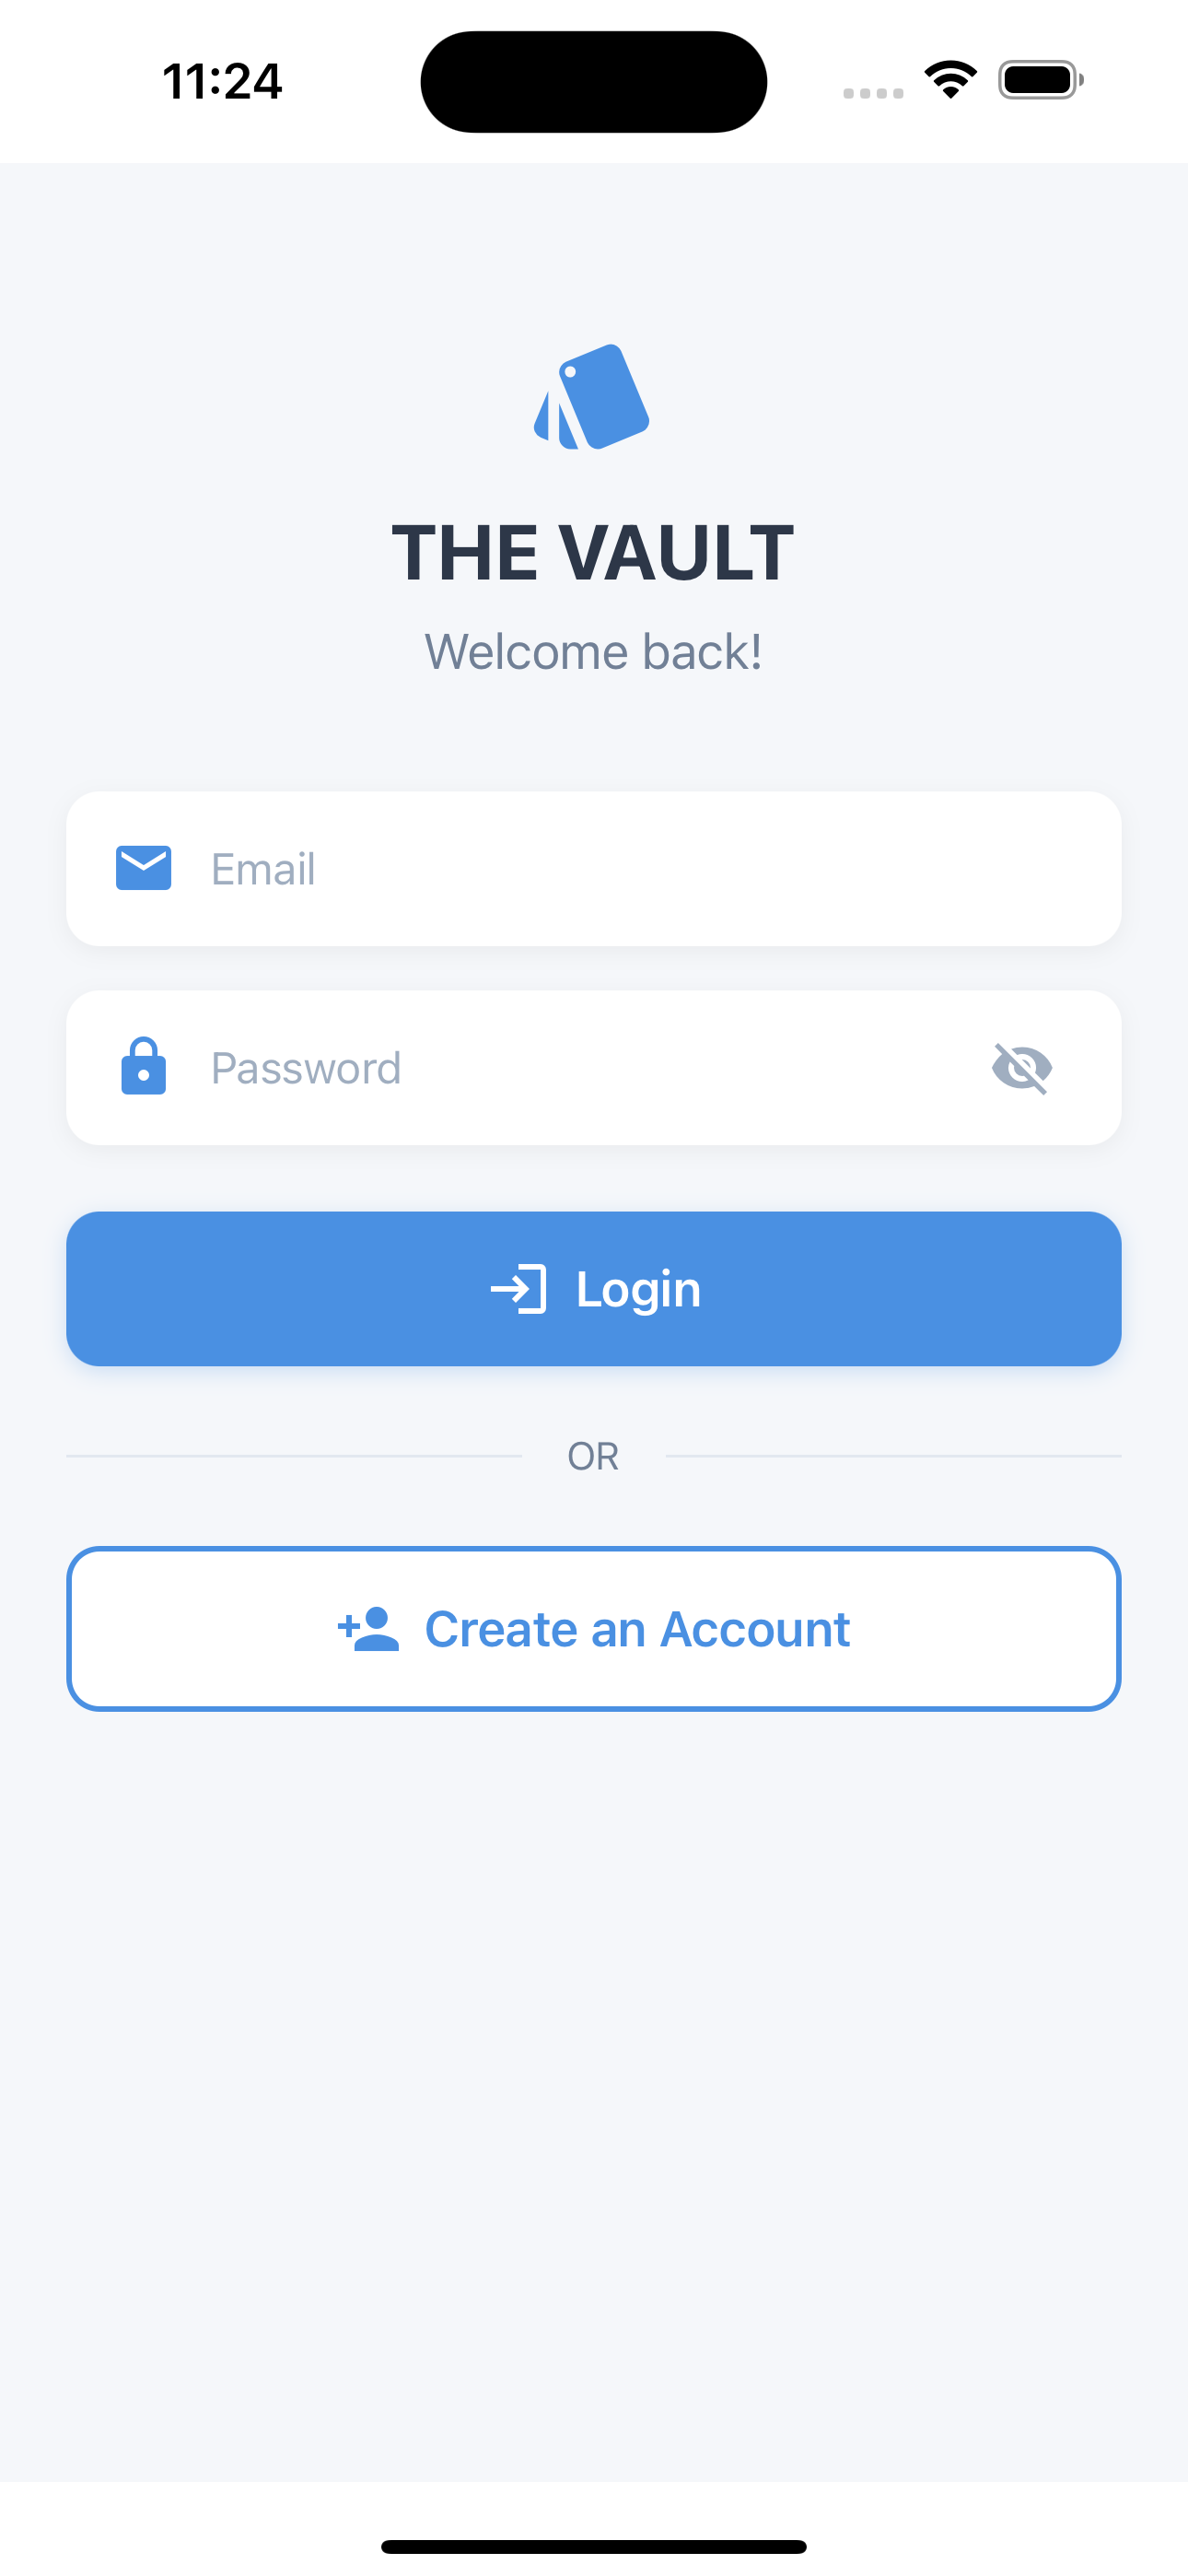
\includegraphics[width=0.3\textwidth]{exampleis-master/figures/loginscreen.png}}
    \qquad % Adds horizontal spacing between the images
    % Second Subfloat: Signup Screen
    \subfloat[Signup screen - new user registration.\label{fig:signup}]
    {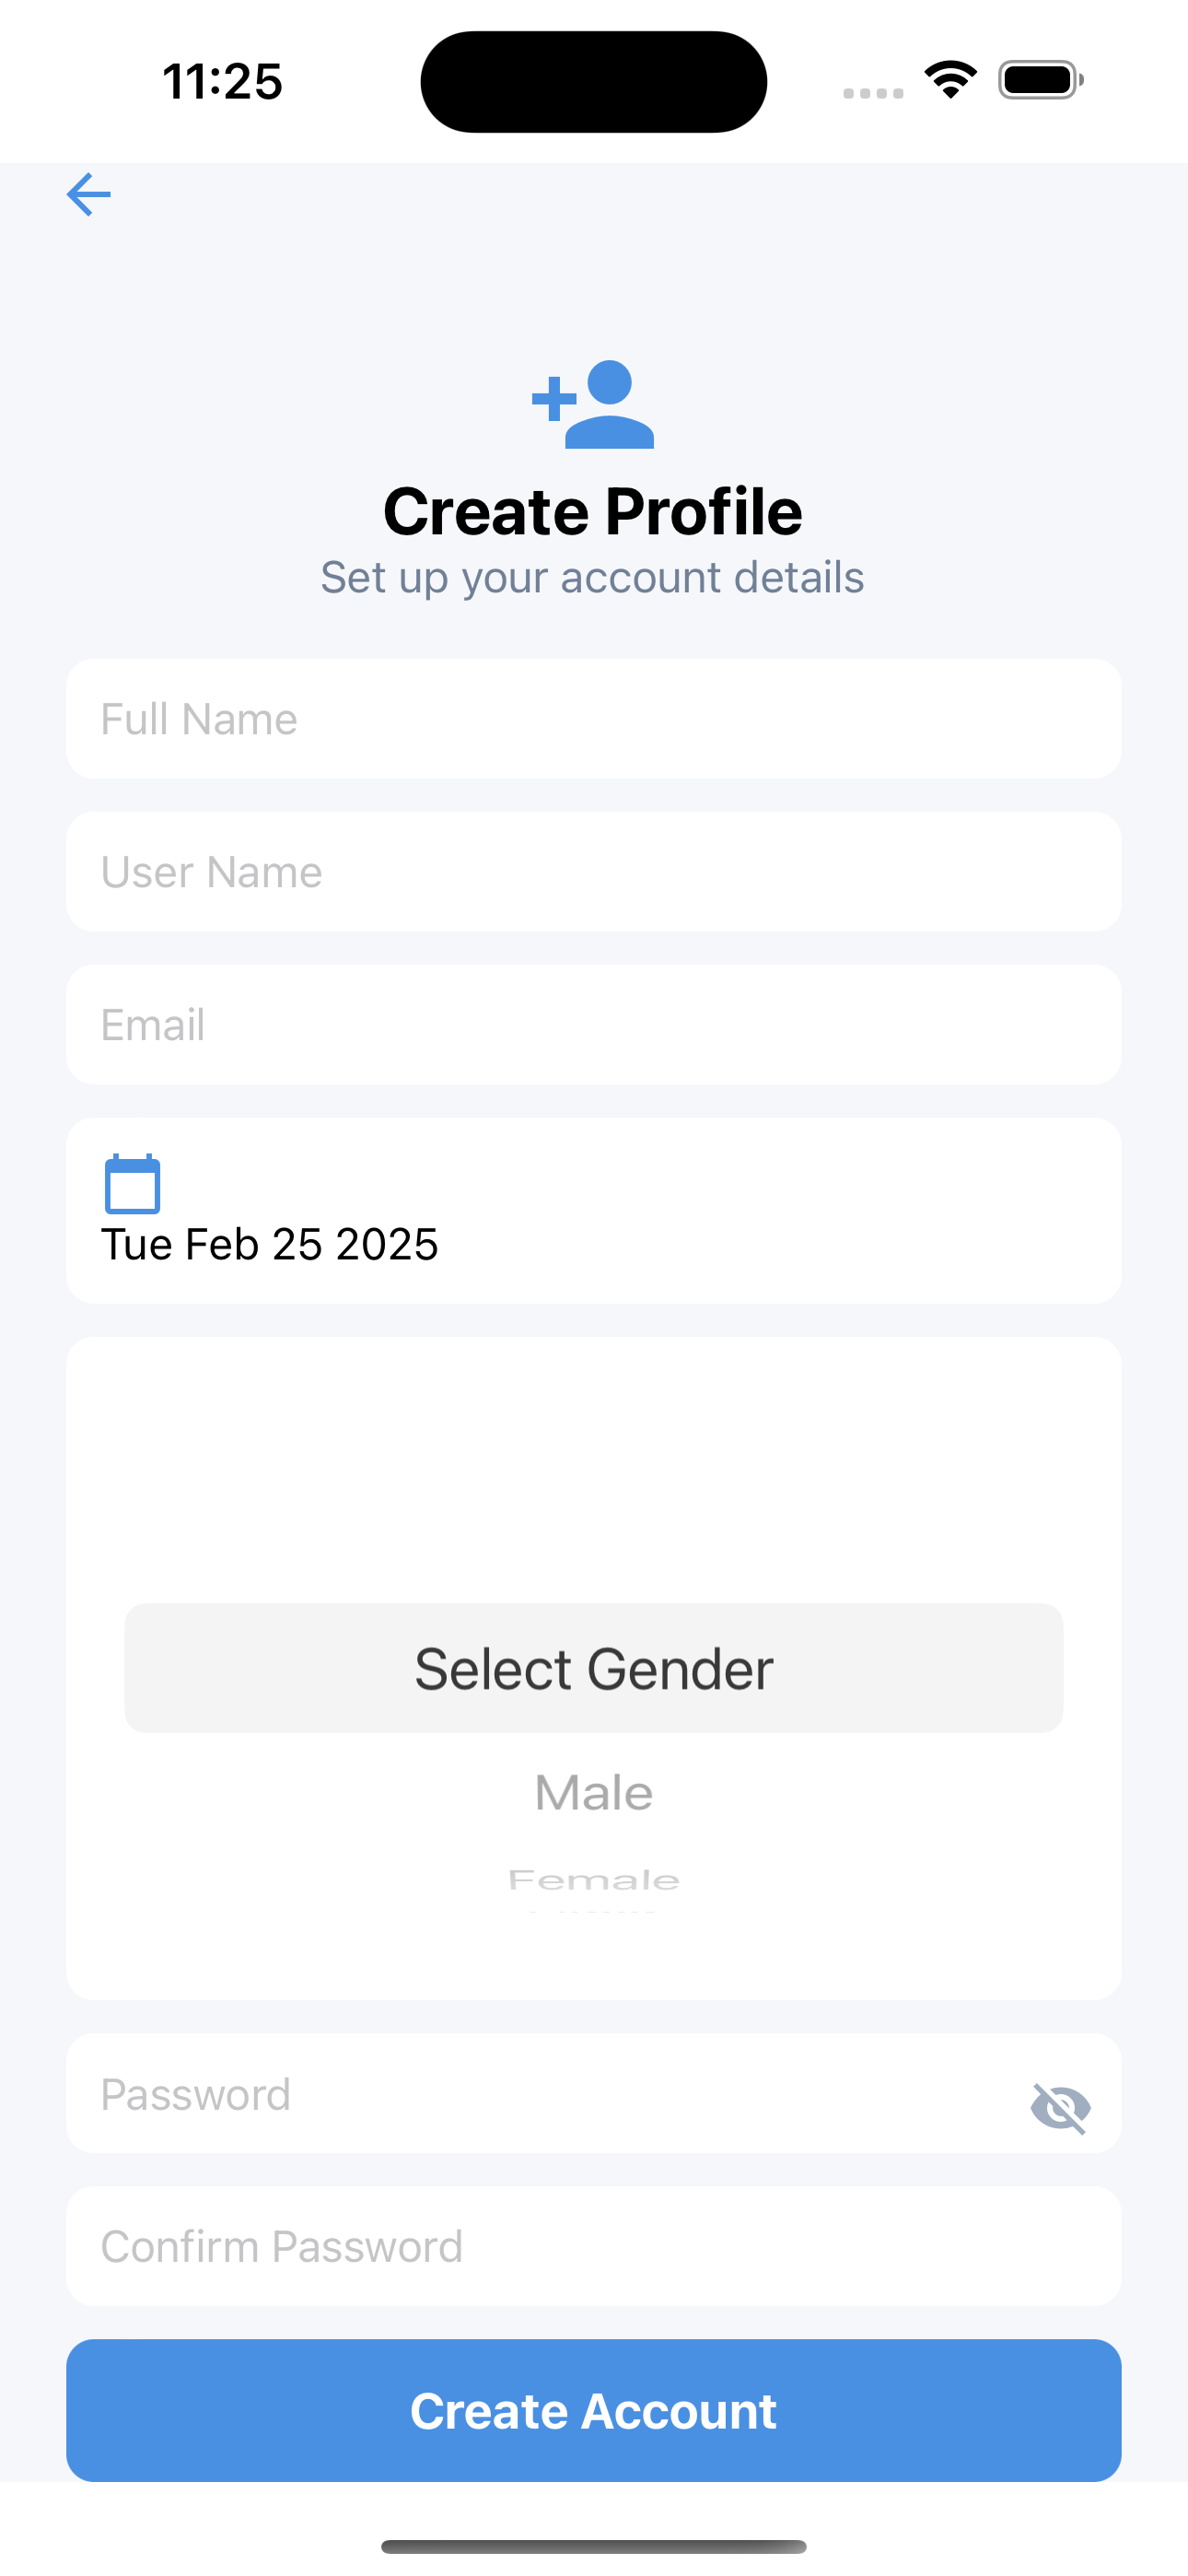
\includegraphics[width=0.3\textwidth]{exampleis-master/figures/signupscreen.png}}
    \caption{Authentication flow: users can sign up for a new account or log in to access their personalized wardrobe.}
    \label{fig:auth_flow}
\end{figure}

This redirection ensures that authenticated users can immediately access their personalized wardrobe without manual navigation. Conversely, if the user is not authenticated \textbf{(Line 17)}, they are redirected to the Login Screen \textbf{(Line 18)} to sign in as shown in Figure \ref{fig:login}. The use of \texttt{router.replace()}also prevents users from navigating back to the login screen after successfully logging in, maintaining a logical and secure flow throughout the app.

\begin{figure}[h]
    \centering
    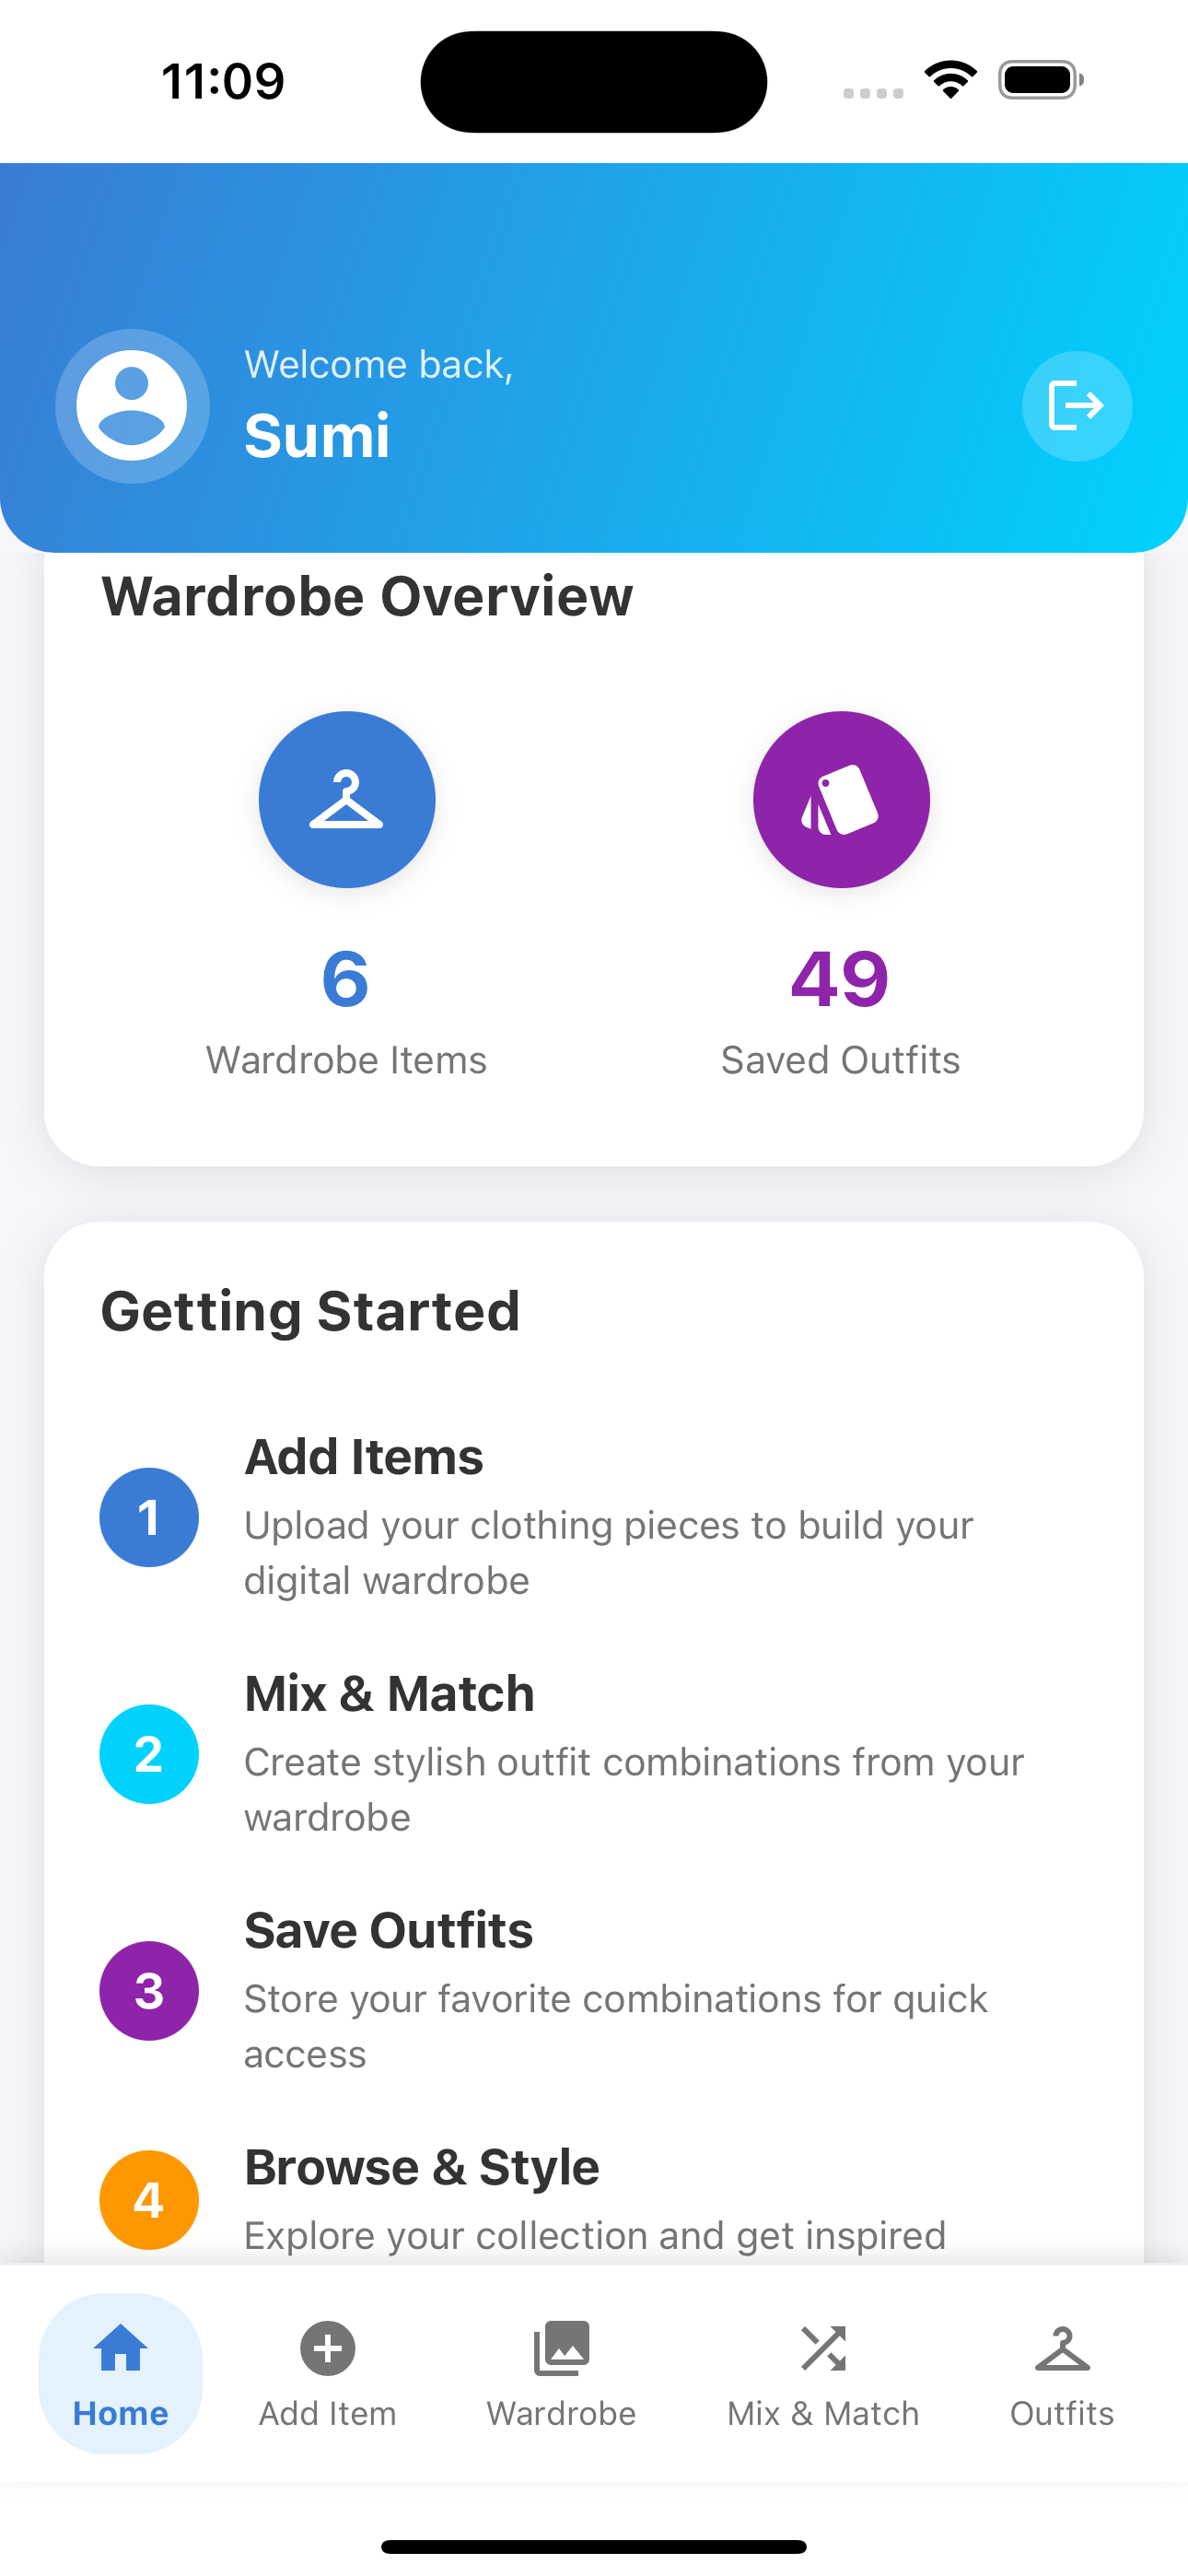
\includegraphics[width=0.3\textwidth]{exampleis-master/figures/homescreen.png}
    \caption{Home screen - user dashboard after successful login}
    \label{fig:home}
\end{figure}


The \texttt{unsubscribe} function \textbf{(Line 20)} returned from \texttt{onAuthStateChanged} ensures that Firebase stops listening for authentication changes when the component is no longer active, improving performance and preventing memory leaks.

Finally, if the authentication check is complete \textbf{(Line 23)} (\texttt{loading} is \texttt{false}), the component returns \texttt{null} \textbf{(Line 27)}, as the routing logic has already directed the user to the appropriate screen. This implementation ensures that the user experience remains smooth, secure, and responsive, with real-time authentication checks providing instant feedback and navigation adjustments based on user actions.


\subsection{Data Management and Storage}
Once a user is authenticated and navigates through the app, My Digital Wardrobe relies on Firebase Cloud Storage and Firestore to handle image uploads and organize wardrobe data. These services work together to ensure that clothing images are securely stored while metadata—such as category, upload date, and user information—remains easily accessible for browsing and outfit creation.

When a user uploads a clothing item, the image file is stored in Firebase Cloud Storage, while Firestore maintains details about the item. This separation ensures that large image files do not slow down database operations, while structured metadata enables quick filtering and retrieval.

The process begins when a user selects an image to upload. The image file is converted into a format suitable for storage, assigned a unique name to prevent overwrites, and uploaded to Firebase Storage. Once the upload is complete, a publicly accessible URL is generated and stored in Firestore along with relevant metadata, as shown in Listing \ref{lst:Firebaseupload}
\begin{lstlisting}[caption={Storing images and metadata in \texttt{Firebaseupload.js}},label=lst:Firebaseupload]
import { ref, uploadBytes, getDownloadURL } from "firebase/storage";
import { collection, addDoc } from "firebase/firestore";
import { storage, db } from "./firebase";

export const uploadImageToFirebase = async (imageUri, category) => {
    const imageName = `${Date.now()}-${imageUri.split("/").pop()}`;
    const storageRef = ref(storage, `wardrobe/${category}/${imageName}`);
    const response = await fetch(imageUri);
    const blob = await response.blob();

    await uploadBytes(storageRef, blob);
    const downloadUrl = await getDownloadURL(storageRef);
    await addDoc(collection(db, "wardrobeItems"), {
        imageUrl: downloadUrl,
        category,
        uploadedAt: new Date(),
    });
};
\end{lstlisting}

This function ensures that every image is stored efficiently while keeping metadata structured for easy retrieval. With Firestore tracking categories such as "Tops" and "Bottoms," wardrobe items are automatically sorted and can be displayed within their respective sections.

Once an item is stored, it becomes accessible through the app’s browsing features. When users navigate to \textbf{WardobeScreen} \ref{fig:wardrobe_screen} , a query to Firestore retrieves the relevant clothing items, grouping them by category. This ensures an easy browsing experience, allowing users to scroll through their wardrobe without delays.

The integration of Firebase services provides a foundation for efficient wardrobe management. Users can upload clothing, categorize items, and retrieve them when needed. This structured approach ensures that wardrobe data remains organized and accessible at all times.


\subsection{Image Uploading and Categorization}

Following user authentication and storing their data, the Upload Screen plays a vital role in My Digital Wardrobe by enabling users to add clothing items from their device’s gallery. Once authenticated and directed to the \textbf{Home Screen} as seen in Figure \ref{fig:home}, users can navigate to the \textbf{Upload Screen} \ref{fig:image_upload_flow}, where they can select and upload images representing their wardrobe items. This functionality is essential for personalizing the wardrobe experience and serves as the starting point for organizing and creating outfits within the app.

The \textbf{Upload Screen} in Figure \ref{fig:gallery_access} provides an intuitive interface where users can select multiple images at once, categorize them into tops and bottoms, and upload them securely. The integration between Expo’s  \texttt{ImagePicker} API and ensures that this process is efficient. Additionally, relevant metadata, mentioned in Chapter \ref{chap:Chapter4} such as category and upload timestamp, is stored in Firestore, allowing for easy organization and retrieval of wardrobe items later.

The core logic for the image uploading feature resides in the \texttt{upload.js} file. The following code snippet in Listing \ref{lst:picker} outlines how \texttt{ImagePicker} and Firebase services collaborate to process and store images:
\begin{lstlisting}[caption={Image picker integration in \texttt{ upload.js}},label=lst:picker]
import * as ImagePicker from "expo-image-picker";
import { uploadImageToFirebase } from "./firebaseUpload";

const pickImages = async (category) => {
    const result = await ImagePicker.launchImageLibraryAsync({ allowsMultipleSelection: true });
    if (!result.canceled) {
        result.assets.forEach(async (asset) => {
            await uploadImageToFirebase(asset.uri, category);
        });
    }
};
\end{lstlisting}

The image uploading process in \textbf{My Digital Wardrobe} begins by importing essential dependencies \textbf{(Lines 1–2)}. The \texttt{ImagePicker} module from Expo allows users to select images from their device’s gallery, forming the core of the Upload Screen's image selection interface. The \texttt{uploadImageToFirebase} function is a custom utility responsible for uploading selected images to Firebase Storage and saving relevant metadata in Firestore. The \texttt{pickImages} function is then defined \textbf{(Line 3)} as an asynchronous function (\texttt{async}), allowing the app to handle time-consuming tasks like image uploads without freezing the user interface. This function accepts a \texttt{category} parameter, ensuring that each uploaded image is linked to a specific user-selected category, supporting the Upload Screen's category selection interface.

The next step involves launching the image picker \textbf{(Line 4)}. The \texttt{launchImageLibraryAsync} function opens the device’s gallery, allowing users to select multiple images at once, thanks to the \texttt{allowsMultipleSelection:true} setting. Figure \ref{fig:gallery_access}  shows this multi-select capability that enhances convenience when users add several wardrobe items simultaneously, contributing to the Upload Screen's multi-select gallery view. Once images are selected, the function checks the selection \textbf{(Line 5)} using the \texttt{if (!result.canceled)} condition to confirm that the user did not cancel the process, reflecting the Upload Screen's cancel/upload confirmation state. If images are present, the app loops through each image \textbf{(Line 6)} using \texttt{result.assets.forEach} for further processing.

The uploading phase follows \textbf{(Line 7)}, where the \texttt{uploadImageToFirebase} function is invoked for each selected image. This function receives the URI (the file location on the user’s device) and its category as parameters. The \texttt{await} keyword ensures that each image is completely uploaded before the next begins, preventing incomplete uploads and supporting the Upload Screen's upload progress feedback. Finally, after all selected images have been processed \textbf{(Line 9)}, the function completes. By this point, all images are securely stored in Firebase Storage, with metadata saved in Firestore for easy retrieval shown in Figure \ref{fig:firestore_collections}. These items are now ready for display in the Gallery Screen, categorized and organized for users to browse, mix, and match when creating outfits.

\begin{figure}[!ht]
    \centering
    % First Subfloat: Upload Screen
    \subfloat[Upload screen - users can upload images from their device.\label{fig:upload_screen}]
    {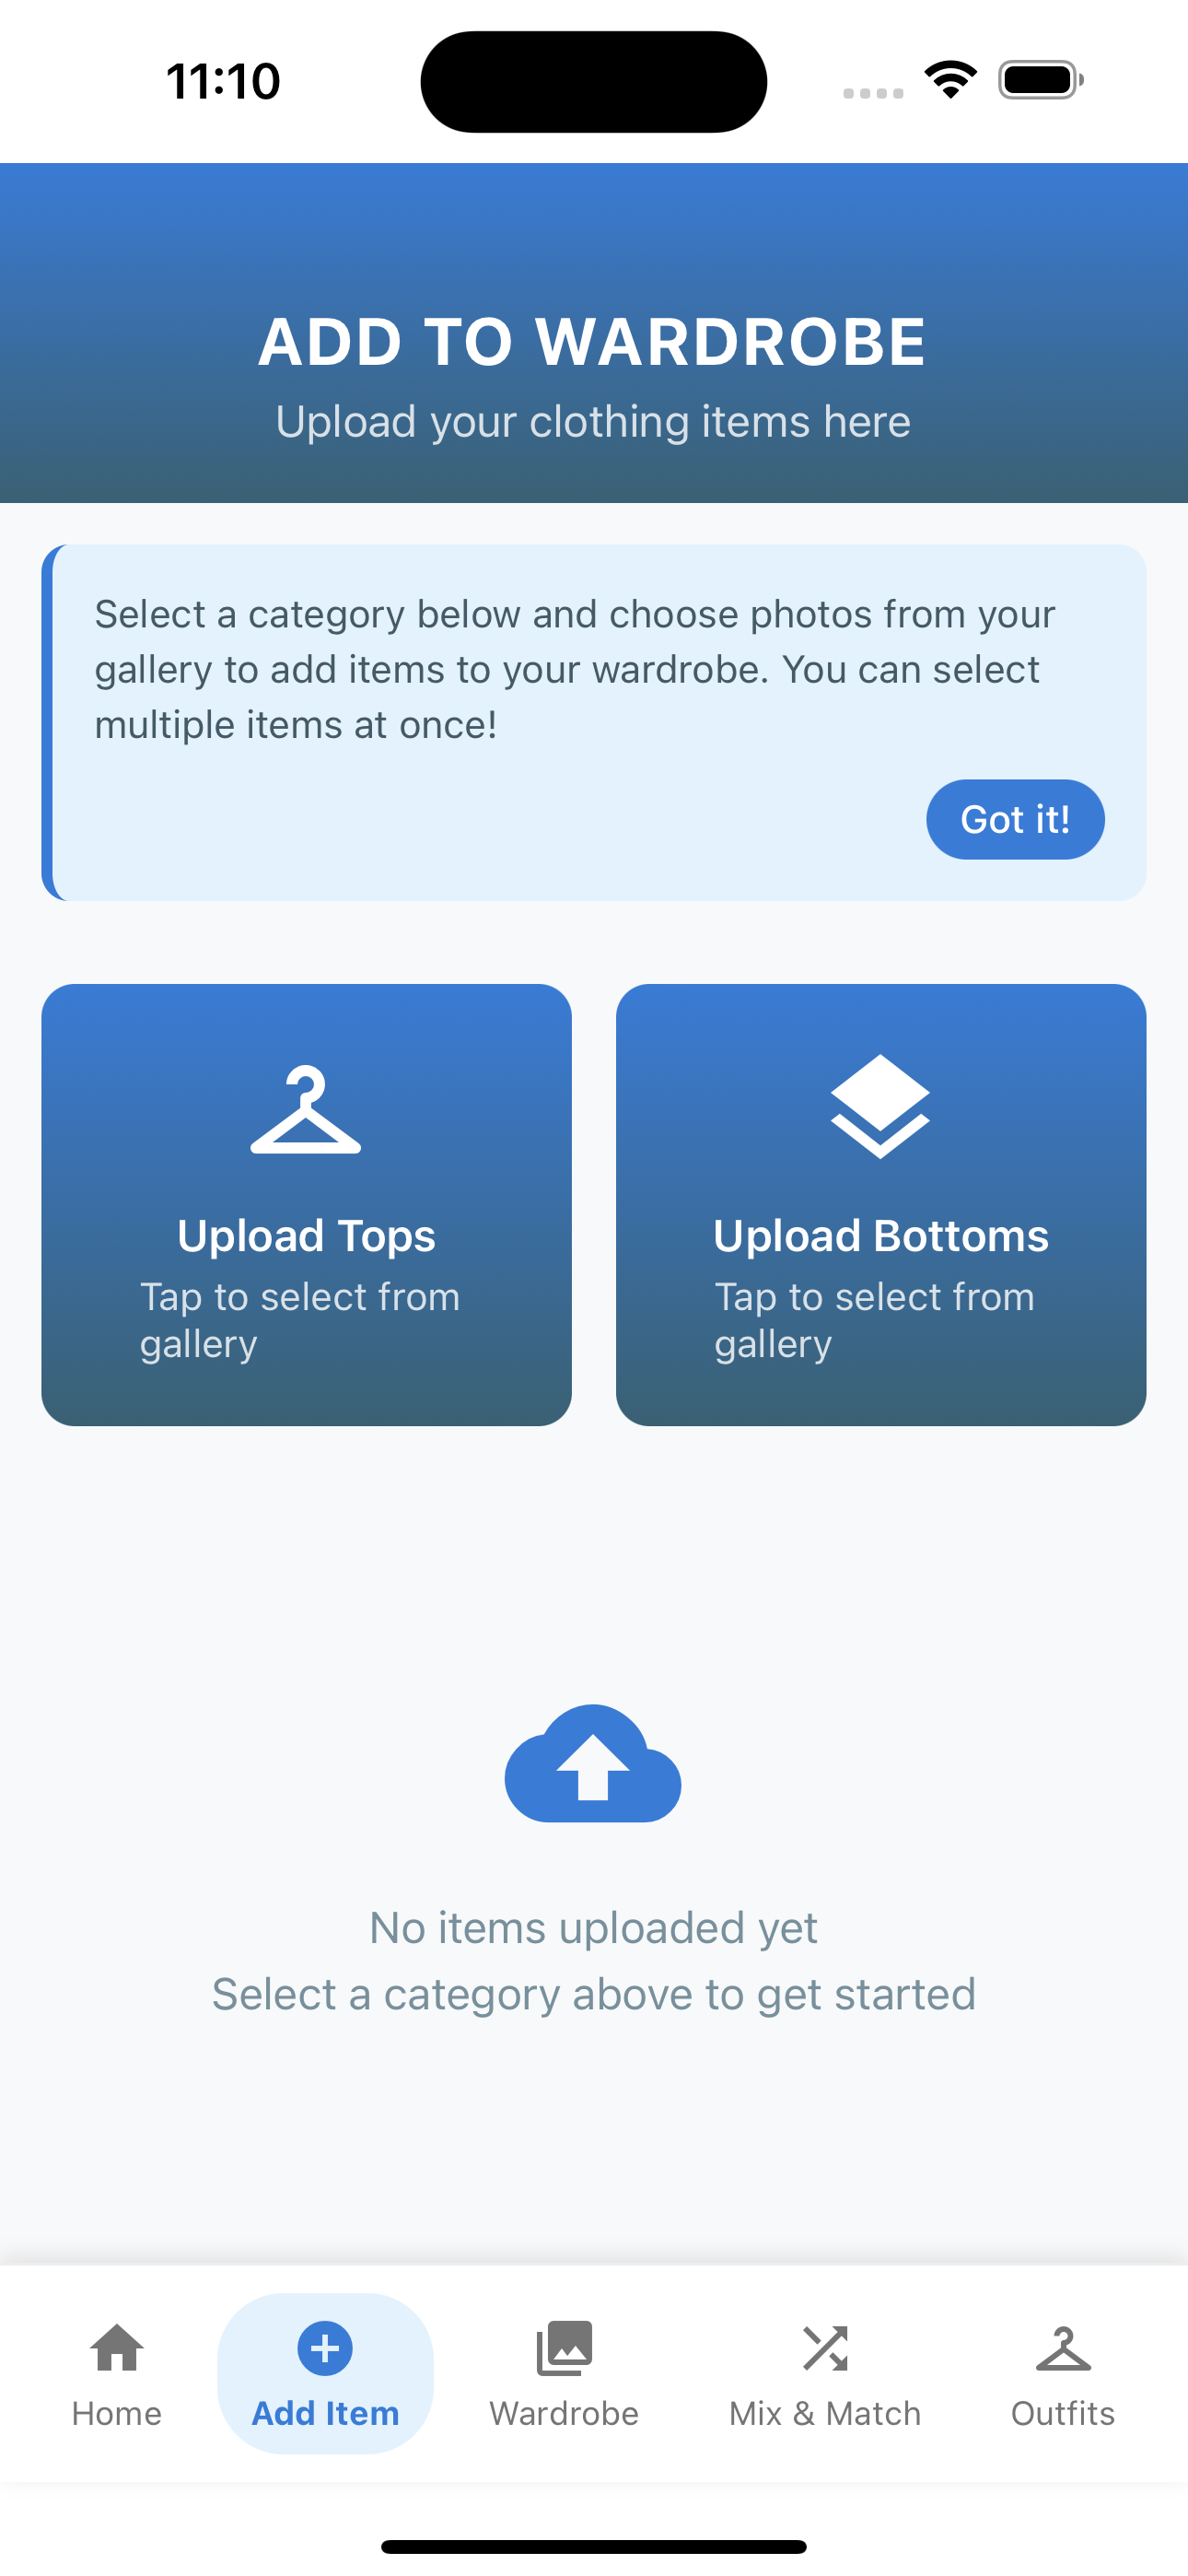
\includegraphics[width=0.3\textwidth]{exampleis-master/figures/uploadscreen.png}}
    \qquad % Adds horizontal spacing between the images
    % Second Subfloat: User Gallery Access Screen
    \subfloat[Gallery access screen - users can select images directly from their device's gallery.\label{fig:gallery_access}]
    {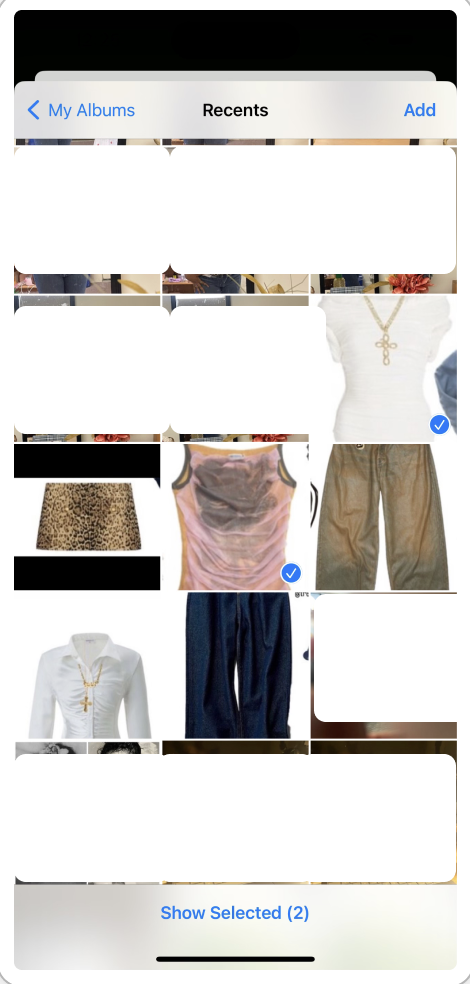
\includegraphics[width=0.3\textwidth]{exampleis-master/figures/defice.png}}
    \caption{Image upload process: users can either upload images directly or access their device's gallery for selection.}
    \label{fig:image_upload_flow}
\end{figure}

Effective wardrobe management in \textit{}{My Digital Wardrobe} is made possible through \textbf{ categorization} and \textbf{interactive browsing}. Users can upload clothing items, assign them to predefined categories, and browse their wardrobe efficiently. These features allow for quick outfit selection, enabling users to mix and match clothing pieces. This section explains how these functionalities are implemented, highlighting their interaction with Firebase and Expo's navigation features.

Each clothing item uploaded to the app is categorized as either a "Top" or a "Bottom" and stored in Firebase Firestore along with its metadata. Categorization simplifies retrieval and filtering, ensuring that users can efficiently browse their wardrobe. The function \texttt{fetchImages}, shown in Listing \ref{lst:fetch_images}, retrieves wardrobe items from Firestore and dynamically assigns them a category.

\begin{lstlisting}[caption={Fetch images by category in \texttt{GalleryScreen.js}}, label={lst:fetch_images}]
const fetchImages = async () => {
    const querySnapshot = await getDocs(collection(db, "wardrobeItems"));
    const itemData = querySnapshot.docs.map((doc) => ({
        ...doc.data(),
        id: doc.id,
        url: doc.data().imageUrl,
        category: doc.data().category?.toLowerCase().includes("top")
            ? "Tops"
            : "Bottoms",
    }));
    setImages(itemData);
};
\end{lstlisting}

This function queries Firestore for all wardrobe items, extracts metadata including the image URL and category, converts category names to lowercase to ensure consistency, and assigns each item to either "Tops" or "Bottoms". The retrieved images are then grouped by category to provide a structured browsing experience, as seen in Listing \ref{lst:group_images}:

\begin{lstlisting}[caption={Group images by category}, label={lst:group_images}]
const groupedImages = images.reduce((acc, item) => {
    if (!acc[item.category]) {
        acc[item.category] = [];
    }
    acc[item.category].push(item);
    return acc;
}, {});
\end{lstlisting}

To enhance user interaction, My Digital Wardrobe incorporates interactive navigation, allowing users to scroll through wardrobe items. Expo's built-in navigation capabilities enable tap selection and horizontal scrolling. The \texttt{handleImageSelect} function, found in Listing \ref{lst:image_select}, enables users to select wardrobe items by tapping.

\begin{lstlisting}[caption={Image selection handler}, label={lst:image_select}]
const handleImageSelect = (item) => {
    if (item.category === "Tops") {
        setSelectedTop(selectedTop?.id === item.id ? null : item);
    } else if (item.category === "Bottoms") {
        setSelectedBottom(selectedBottom?.id === item.id ? null : item);
    }
};
\end{lstlisting}

This implementation allows users to tap an item to select it, tap again to deselect it, and independently choose tops and bottoms before creating an outfit. A visual cue is provided to indicate selected items as demonstarted in Figure \ref{fig:selection_ visual_aid}. Conditional styling in Listing \ref{lst:selected_style} highlights selections with a colored border.

\begin{lstlisting}[caption={Conditional styling for selected items}, label={lst:selected_style}]
const styles = StyleSheet.create({
    selectedImage: {
        borderWidth: 3,
        borderColor: "#FF1493",
    },
});
\end{lstlisting}

\begin{figure}[!ht]
    \centering
    % First Subfloat: Warbrobe Screen
    \subfloat[Wardrobe screen - displays categorized wardrobe items.\label{fig:wardrobe_screen}]
    {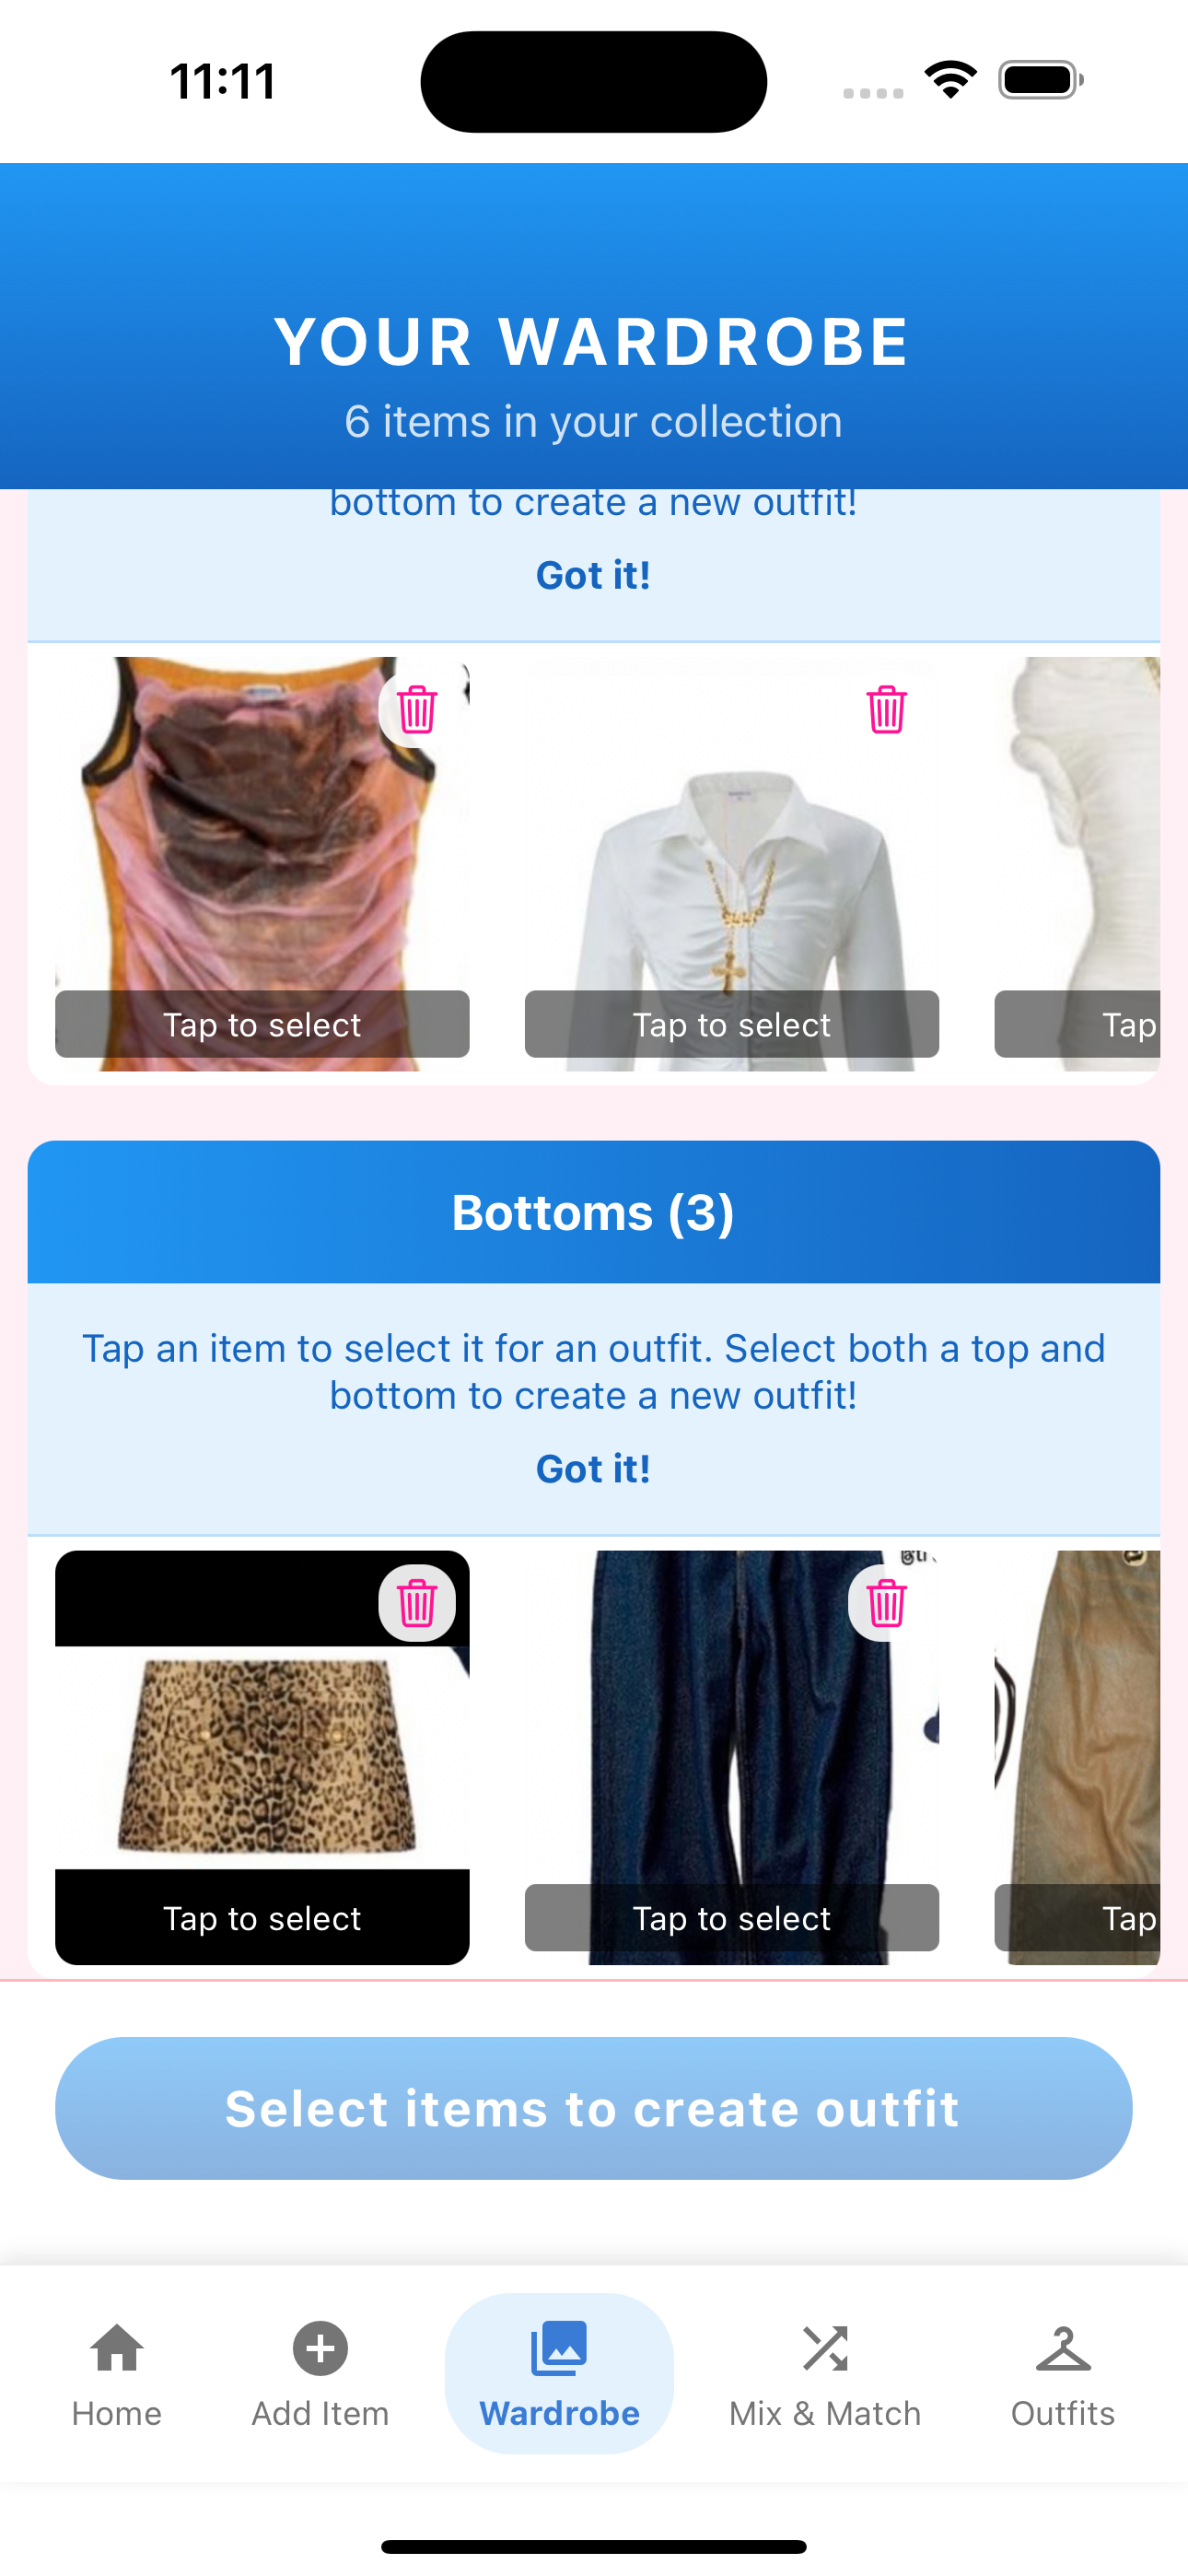
\includegraphics[width=0.3\textwidth]{exampleis-master/figures/wardrobe1.png}}
    \qquad % Adds horizontal spacing between the images
    % Second Subfloat: Outfit Screen
    \subfloat[Warbrobe screen - users can see thier selection.\label{fig:cameraroll_screen}]
    {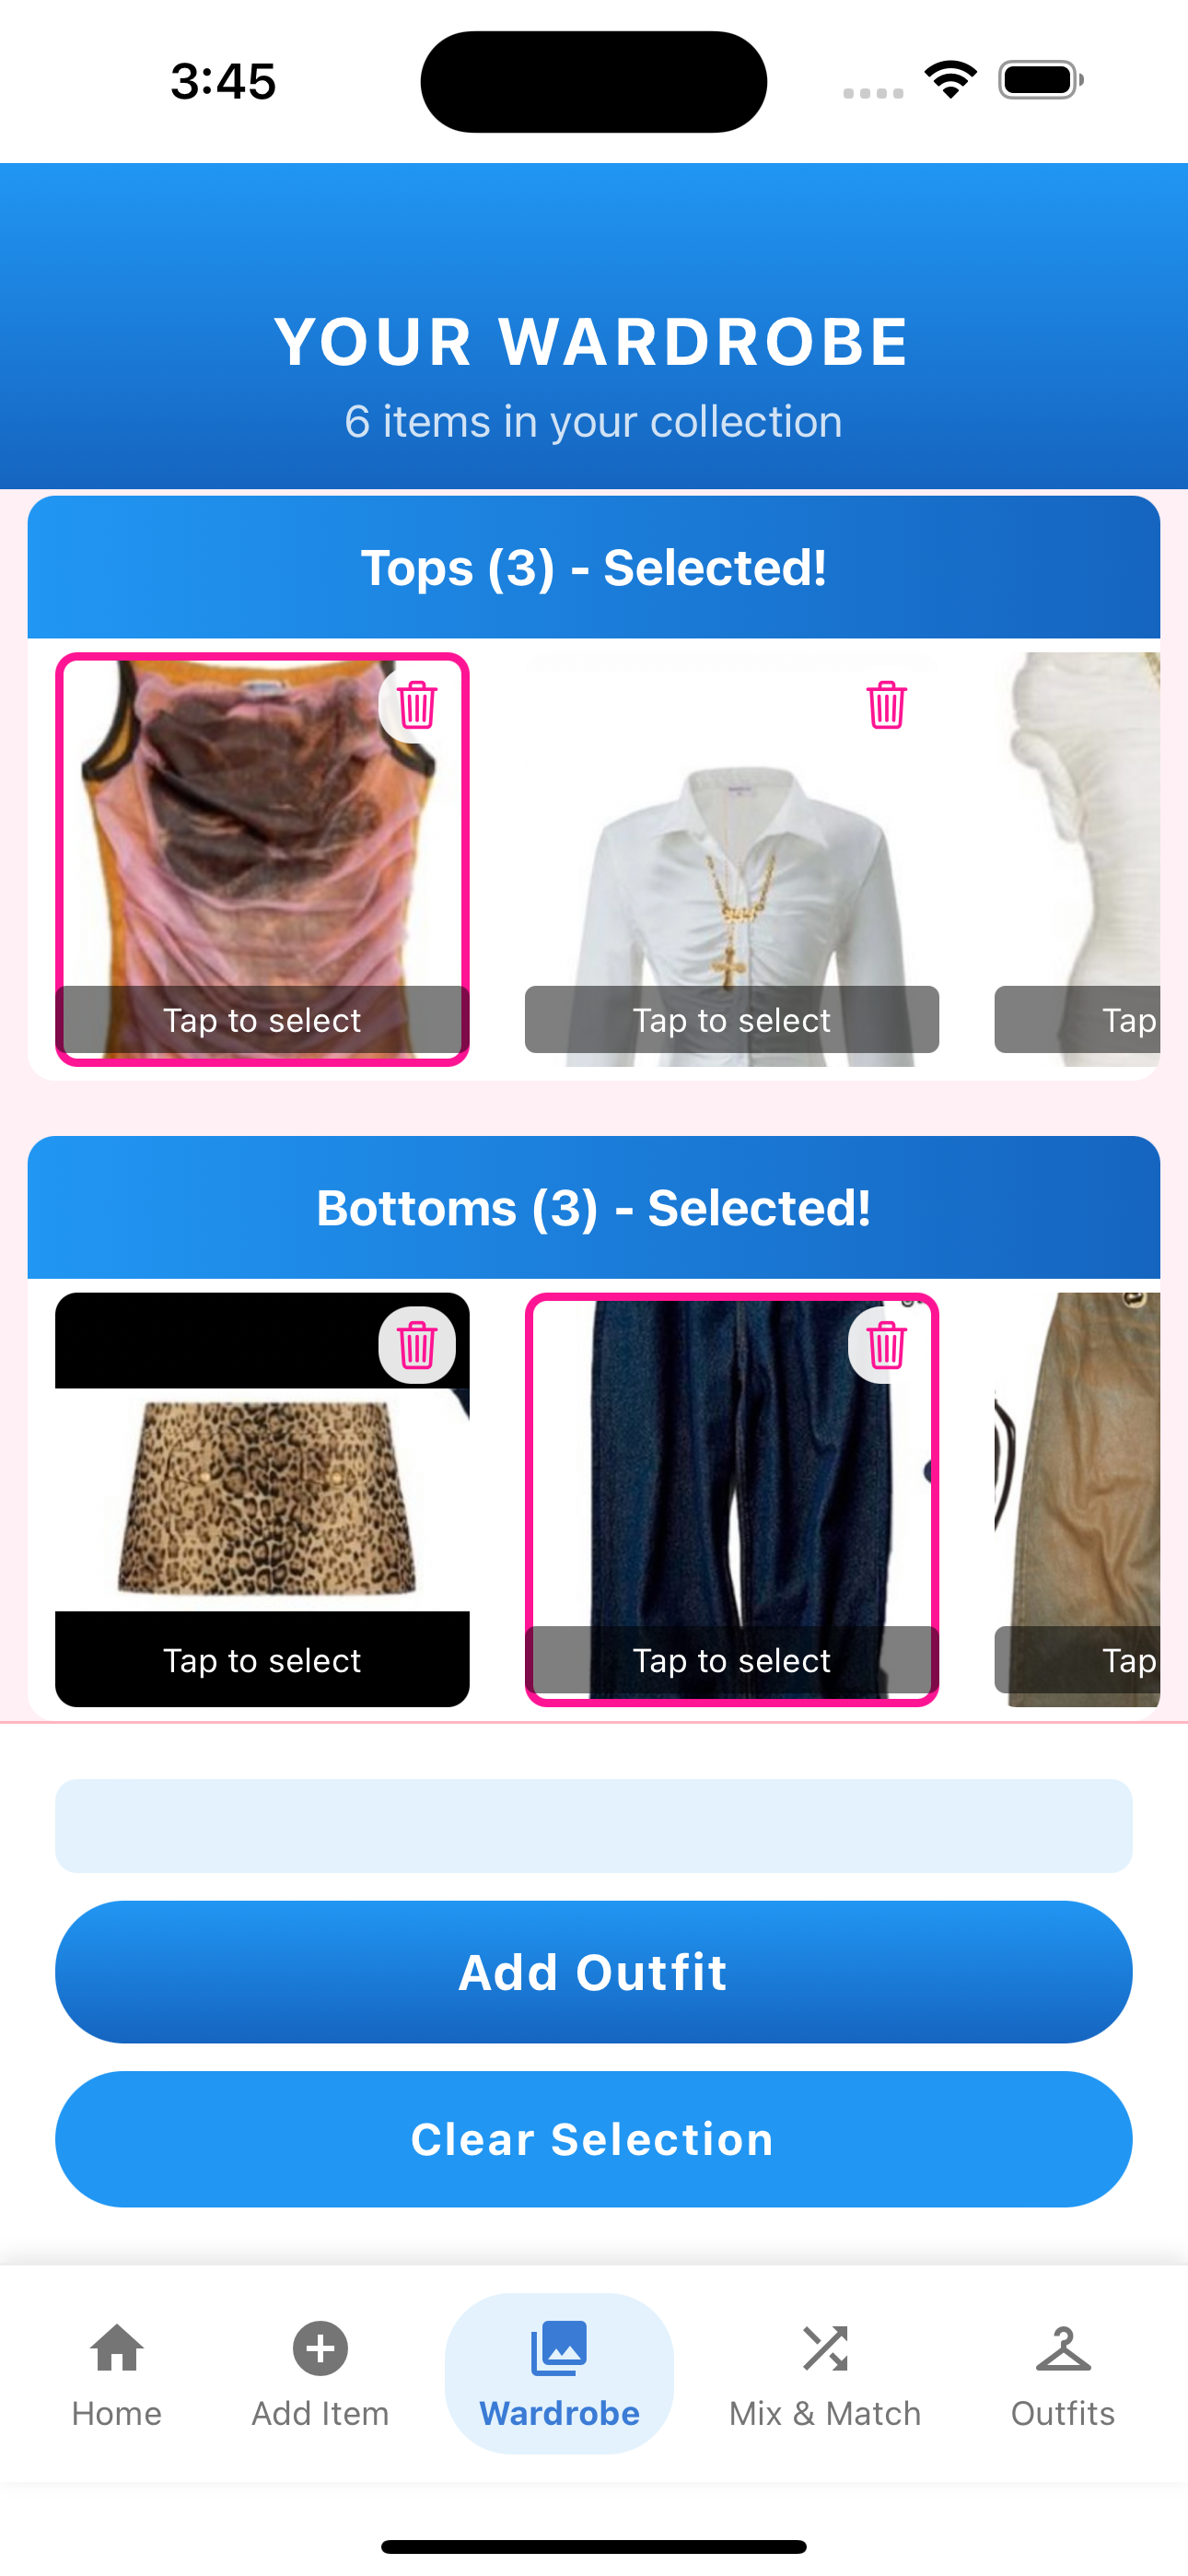
\includegraphics[width=0.3\textwidth]{exampleis-master/figures/wardrobe3.png}}
    \caption{Wardrobe browsing and outfit management: users can browse their categorized wardrobe in the wardrobe screen and add their selection}
    \label{fig:selection_ visual_aid}
\end{figure}

Once users have selected a top and bottom, they can preview the combination in OutfitScreen as shown in Figure \ref{fig:cameraroll_screen}. The function \texttt{renderOutfitCard} in Listing \ref{lst:outfit_card} dynamically displays selected outfit items.

\begin{lstlisting}[caption={Render outfit card in \texttt{OutfitScreen.js}}, label={lst:outfit_card}]
const renderOutfitCard = ({ item }) => (
    <View style={styles.outfitCard}>
        <Image source={{ uri: item.top }} style={styles.outfitImage} />
        <Image source={{ uri: item.bottom }} style={styles.outfitImage} />
        <Text>{item.name || "Untitled Outfit"}</Text>
    </View>
);
\end{lstlisting}

This preview ensures that users can visually assess outfit combinations before saving them. The function handleSaveOutfit in Listing \ref{lst:save_outfit}, also found in OutfitScreen.js, stores the finalized selection in Firestore.

\begin{lstlisting}[caption={Save outfit function}, label={lst:save_outfit}]
const handleSaveOutfit = async () => {
    const selectedTop = wardrobe.tops[selectedTopIndex];
    const selectedBottom = wardrobe.bottoms[selectedBottomIndex];
    await saveOutfit({ top: selectedTop, bottom: selectedBottom });
};
\end{lstlisting}

This step ensures that saved outfits can be accessed later in the Outfit Screen, where users can delete or manage their stored combinations.

Additionally, a randomization feature has been implemented as seen in Listing \ref{lst:randomize_outfit}, allowing users to generate outfit combinations automatically. This feature selects a random top and bottom from the wardrobe:

\begin{lstlisting}[caption={Randomize outfit function}, label={lst:randomize_outfit}] 
const handleRandomize = () => {
    setSelectedTopIndex(Math.floor(Math.random() * wardrobe.tops.length));
    setSelectedBottomIndex(Math.floor(Math.random() * wardrobe.bottoms.length));
};
\end{lstlisting}

\begin{figure}[!ht]
    \centering
    % First Subfloat: Warbrobe Screen
    \subfloat[Mix and match screen - displays selected items from Wardrobe.\label{fig:mixandmatch_screen}]
    {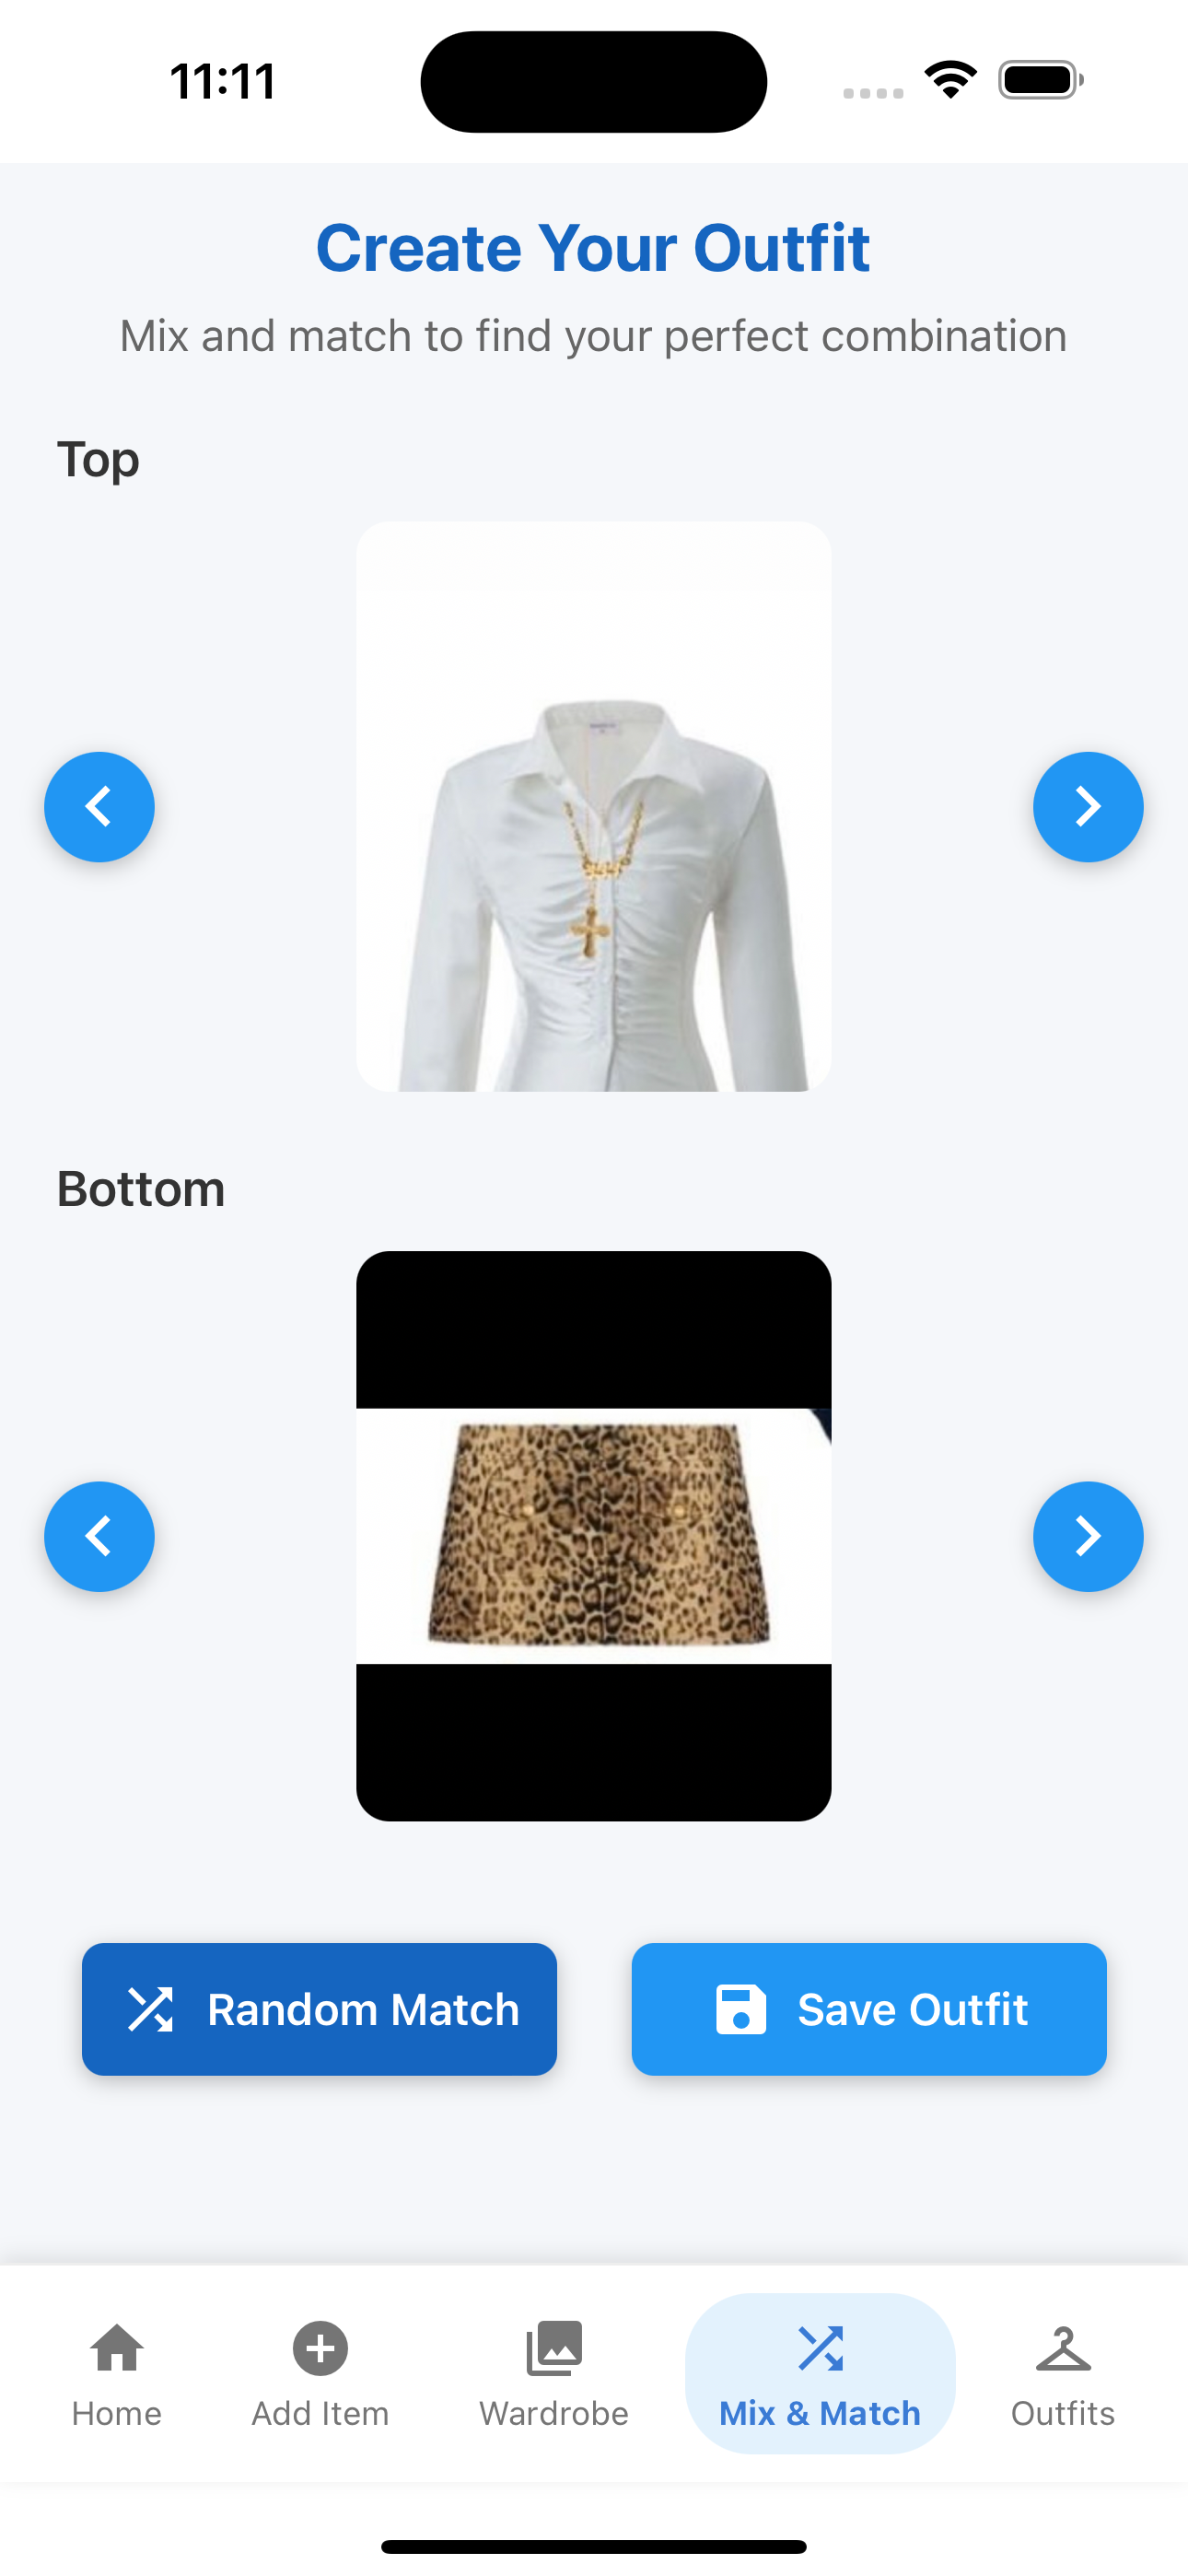
\includegraphics[width=0.3\textwidth]{exampleis-master/figures/mixandmatch.png}}
    \qquad % Adds horizontal spacing between the images
    % Second Subfloat: Outfit Screen
    \subfloat[Outfit screen - users can view and manage saved outfits.\label{fig:outfit_screen}]
    {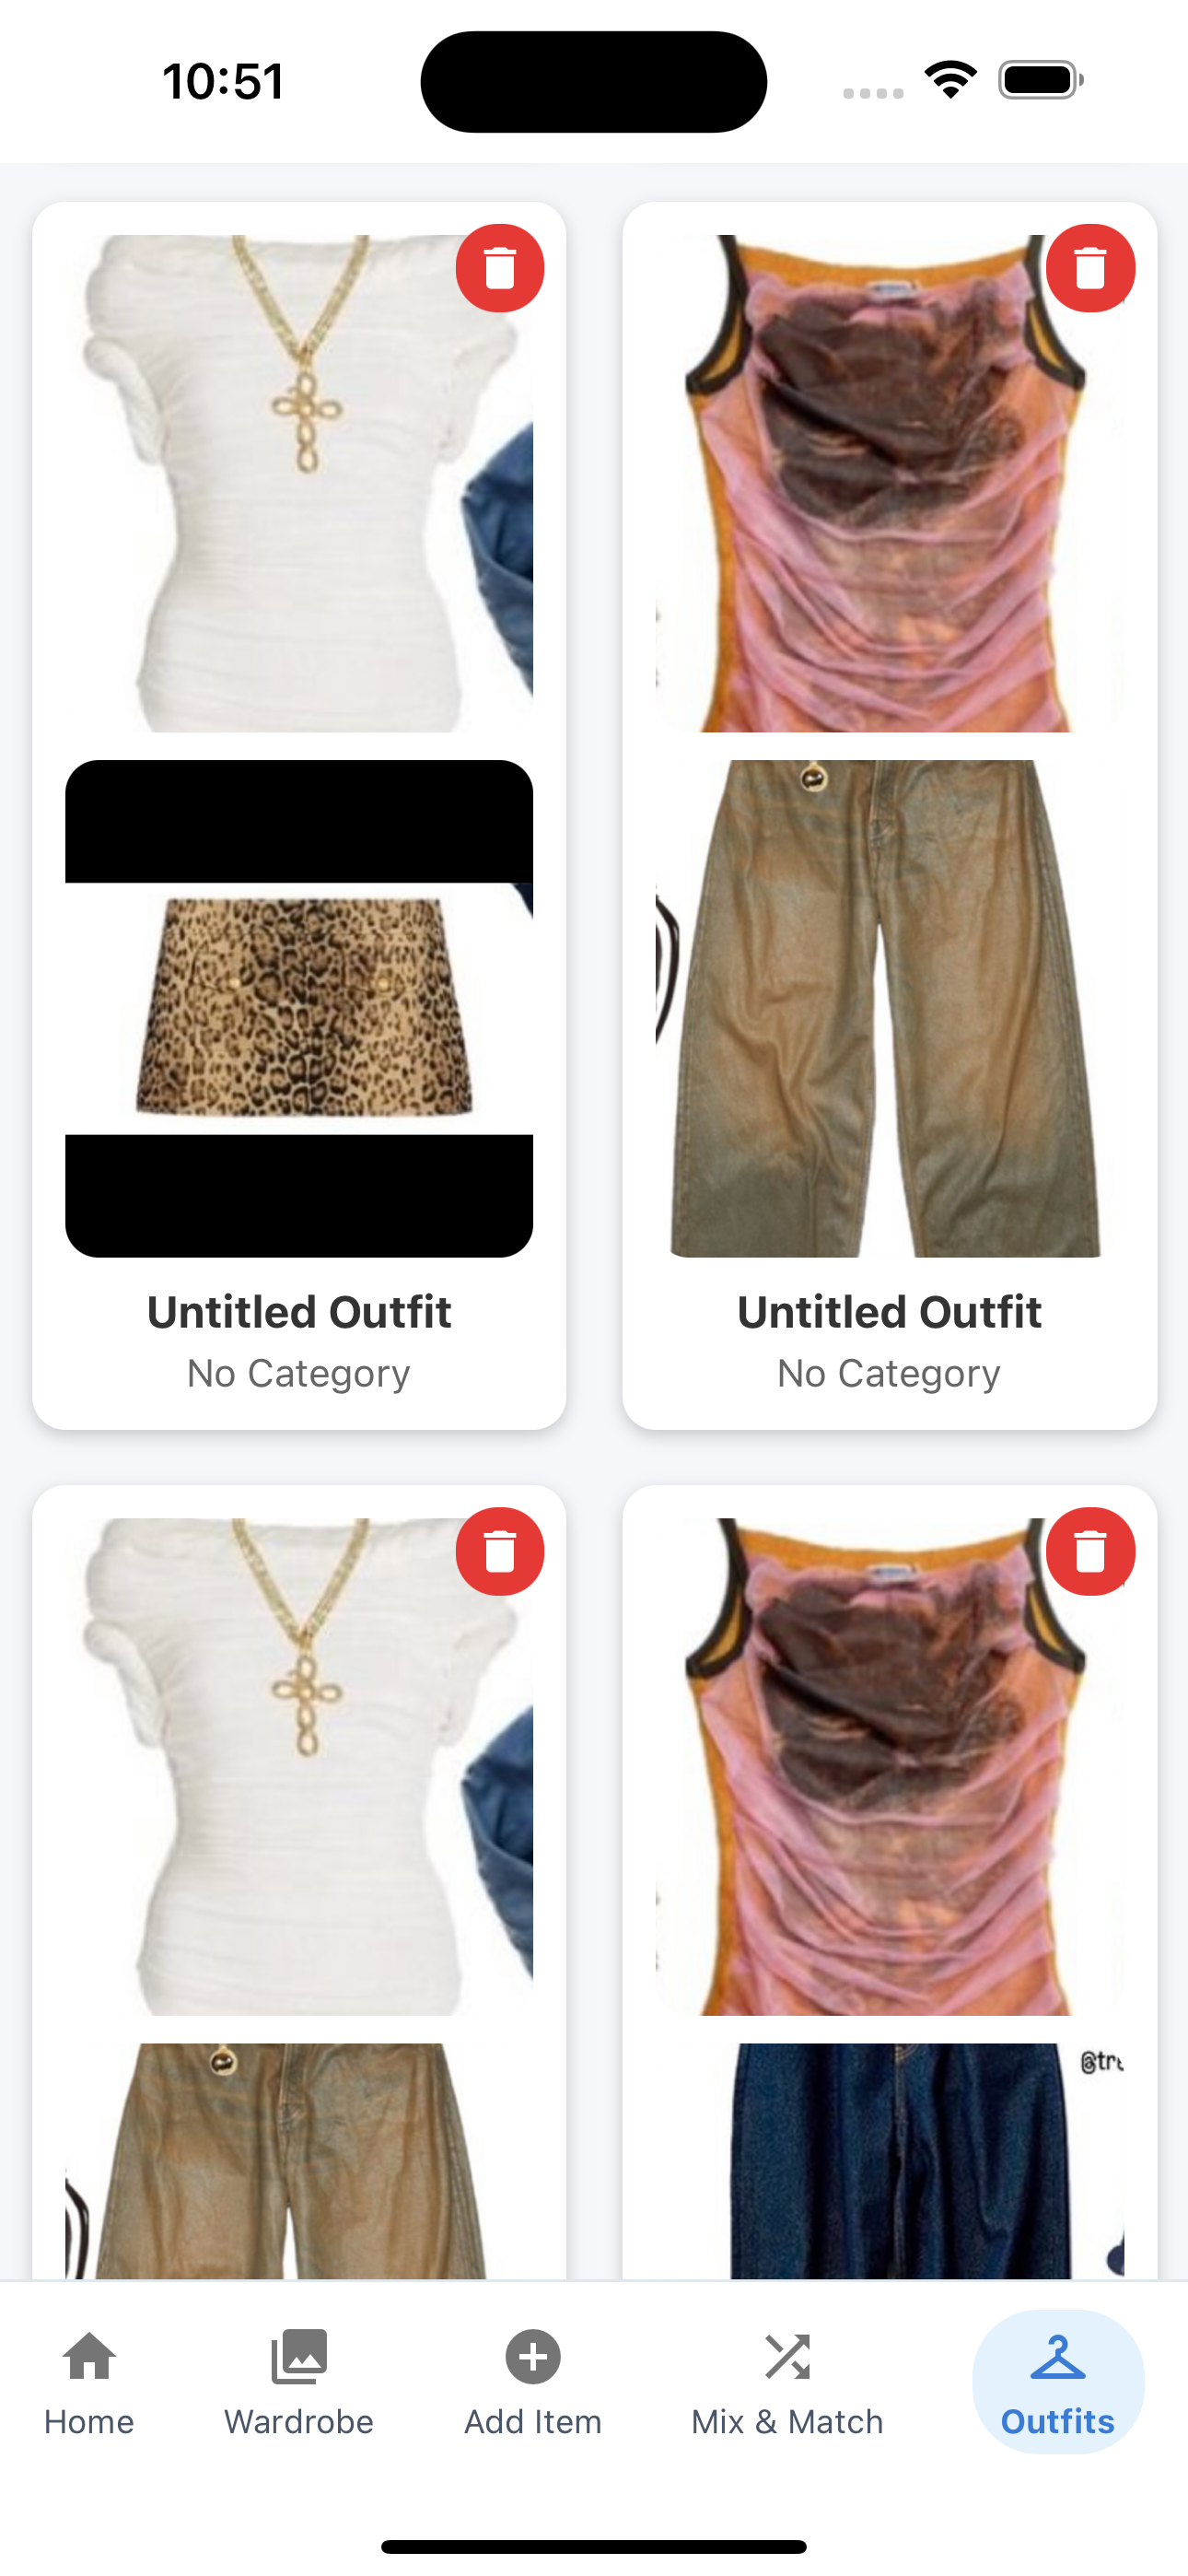
\includegraphics[width=0.3\textwidth]{exampleis-master/figures/outfitscreen2.png}}
    \caption{Outfit creation and saving: users can browse their saved outfits in the mix and match screen and view saved outfits in the outfit screen.}
    \label{fig:wardrobe_outfit_flow}
\end{figure}

By integrating categorization, interactive browsing, and dynamic previews, My Digital Wardrobe provides an intuitive wardrobe management experience. Users can filter through their collection, mix and match outfits, and save preferred combinations for future reference. Figure \ref{fig:mixandmatch_screen} shows how categorized wardrobe items are displayed and selected, while Figure \ref{fig:outfit_screen} demonstrates the saved outfit interface.
With images securely stored and categorized, the next step is allowing users to upload and manage their wardrobe items effectively. 
These features streamline wardrobe organization, making it easy for users to manage and experiment with their clothing selections.

\section{Component Communication}

\textit{My Digital Wardrobe} is built as a collection of interconnected components, each responsible for a specific function within the app. These components handle everything from user authentication to outfit creation, working together to create an intuitive experience. In the previous section we discussed how  certain implementations work along with visual aid, this section provides a step-by-step walkthrough of how the components communicate behind the scenes, ensuring that every action a user takes leads to a meaningful response.

At the heart of the app’s functionality is the way components interact with Firebase. Each time a user logs in, uploads an image, or saves an outfit, data is sent to Firebase services, which stores and manages this information. Expo Router handles navigation, directing users to the appropriate screens based on their actions. This structure ensures that the app remains responsive and dynamic, allowing users to interact with their wardrobe in a natural way.

\begin{table}[h]
    \centering
    \begin{tabular}{|l|l|p{5cm}|}
        \hline
        \textbf{File} & \textbf{Interacts With} & \textbf{Purpose} \\
        \hline
        \texttt{index.js} & \texttt{firebase.js} & Initializes authentication and manages user navigation based on authentication status. \\
        \hline
        \texttt{firebaseUpload.js} & \texttt{firebase.js}, \texttt{upload.js} & Handles image uploads to Firebase Storage and metadata storage in Firestore. \\
        \hline
        \texttt{upload.js} & \texttt{firebaseUpload.js} & Provides the interface for selecting, uploading, and categorizing wardrobe items. \\
        \hline
        \texttt{GalleryScreen.js} & \texttt{firestore.js}, \texttt{OutfitScreen.js} & Displays categorized wardrobe items fetched from Firestore. \\
        \hline
        \texttt{OutfitScreen.js} & \texttt{firebase.js}, \texttt{outfitfirestore.js} & Allows users to view saved outfits or create new outfits by mixing and matching wardrobe items. \\
        \hline
        \texttt{MixAndMatchScreen.js} & \texttt{outfitfirestore.js} & Enables users to select tops and bottoms, check color coordination, and save custom outfits to Firestore. \\
        \hline
    \end{tabular}
    \caption{Component interactions in my digital wardrobe}
    \label{tab:component_communication}
\end{table}

\subsection{Communication Flow}
The user journey begins the moment they open the app. When the app launches, \texttt{index.js} checks whether the user is already logged in. If authentication is successful, they are directed to the \texttt{HomeScreen} as shown in Figure \ref{fig:home}, where they can access different features. If not, they are taken to \texttt{LoginScreen} from Figure \ref{fig:login}, where they must enter their credentials before proceeding.
Once authenticated, the home screen serves as the main entry point. From here, users can choose to upload new clothing items, browse their wardrobe, mix and match outfits, or review previously saved outfits. Each screen is connected to the others through navigation events, ensuring that users can move fluidly between different sections.

When a user selects the option to add a new item, they are taken to \texttt{UploadScreen} in Figure \ref{fig:upload_screen}. This screen allows them to pick images from their device’s gallery and assign them to a category—either “Tops” or “Bottoms.” The selected image is then uploaded to Firebase Storage, while metadata such as category and upload timestamp is stored in Firestore.

The upload process happens in the background, ensuring that users can continue interacting with the app without delays. Once the upload is complete, the wardrobe is updated, and the new item appears in \texttt{GalleryScreen} from Figure \ref{fig:wardrobe_screen}, where it is sorted based on its assigned category.


In \texttt{GalleryScreen}, users can see all the clothing items they have uploaded, organized into their respective categories. When they tap on an item, it is highlighted, indicating that it has been selected. If they wish to create an outfit, they can navigate to \texttt{MixAndMatchScreen} from Figure \ref{fig:mixandmatch_screen}, where they can pair different tops and bottoms to find the best combination.

This screen presents a scrolling view of wardrobe items, allowing users to browse through their collection. They can manually select items or use the randomization feature to generate outfit suggestions. This interaction mimics the experience of flipping through a physical wardrobe, making outfit selection both simple and engaging.

Once a user has found a combination they like, they can save the outfit. This action sends the selected top and bottom to Firestore, where it is stored as a new outfit entry. Saved outfits can be accessed later in OutfitScreen in Figure \ref{fig:outfit_screen}, where users can review, edit, or delete them.

The outfit screen presents saved combinations in a structured layout, ensuring that users can quickly browse their past selections. If they decide to modify an outfit, they can return to MixAndMatchScreen in Figure \ref{fig:mixandmatch_screen} and make adjustments. This creates a continuous loop, where users can experiment with different styles, save their favorites, and revisit them whenever needed.


Every screen in My Digital Wardrobe is designed to respond to user actions, creating an easy interaction flow. Table \ref{tab:component_communication} shows a short summary of these interactions.


